% Native editable composition from verified, unchanged IDE images.
\par
\begin{figure}[htbp]
\centering
\sbox0{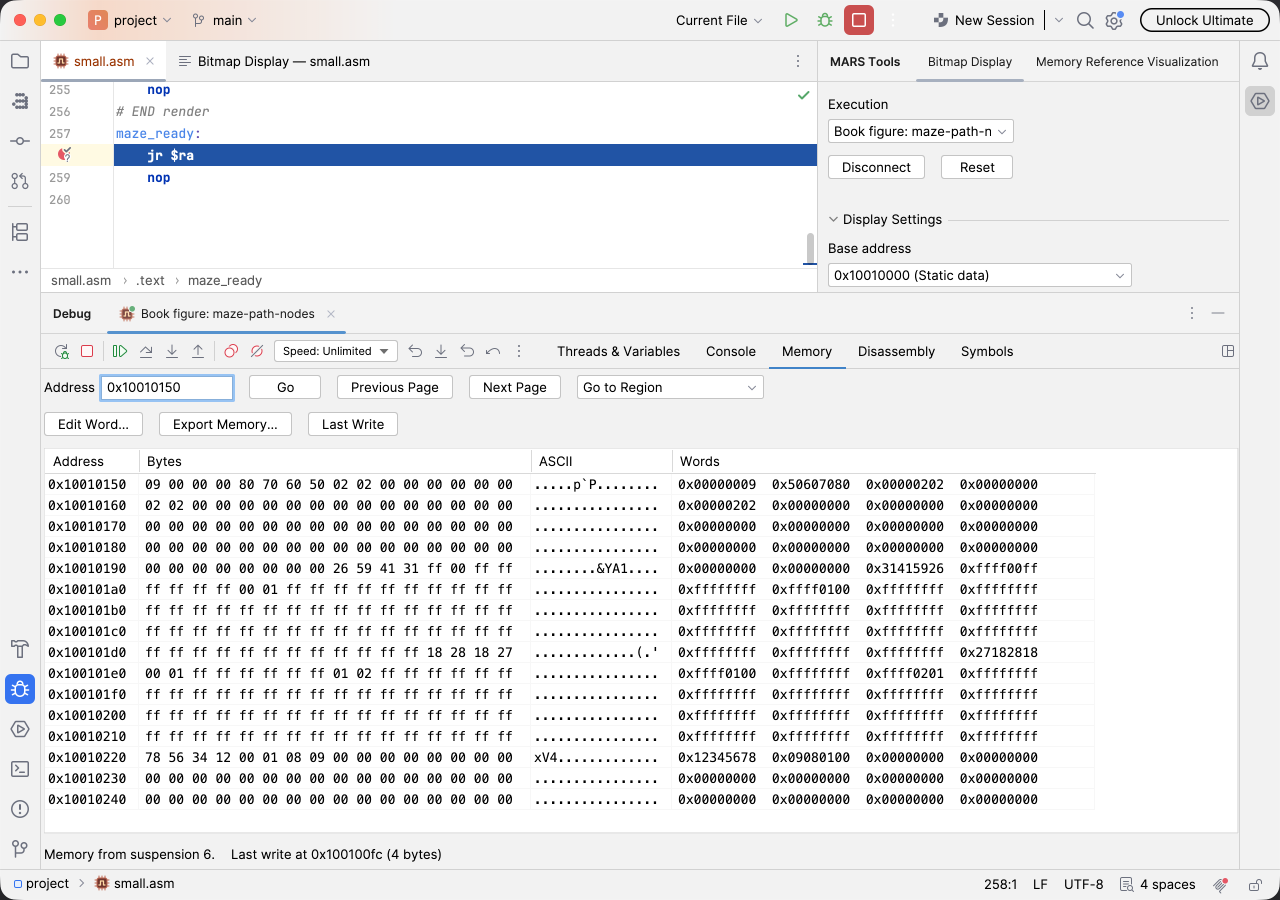
\includegraphics[artifact]{book/captures/010-maze-explorer/f03-path/nodes.png}}
\sbox2{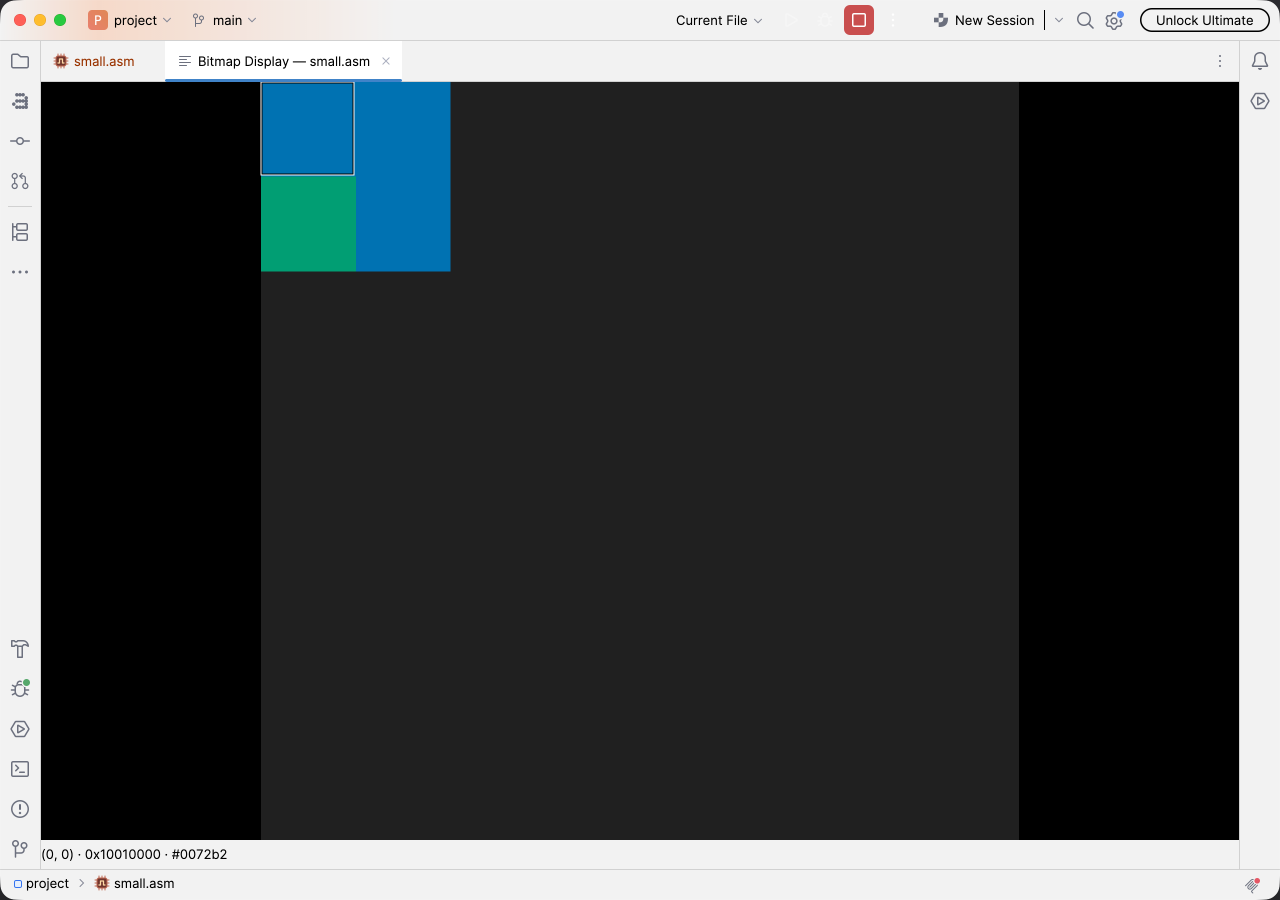
\includegraphics[artifact]{book/captures/010-maze-explorer/f03-path/bitmap.png}}
\sbox4{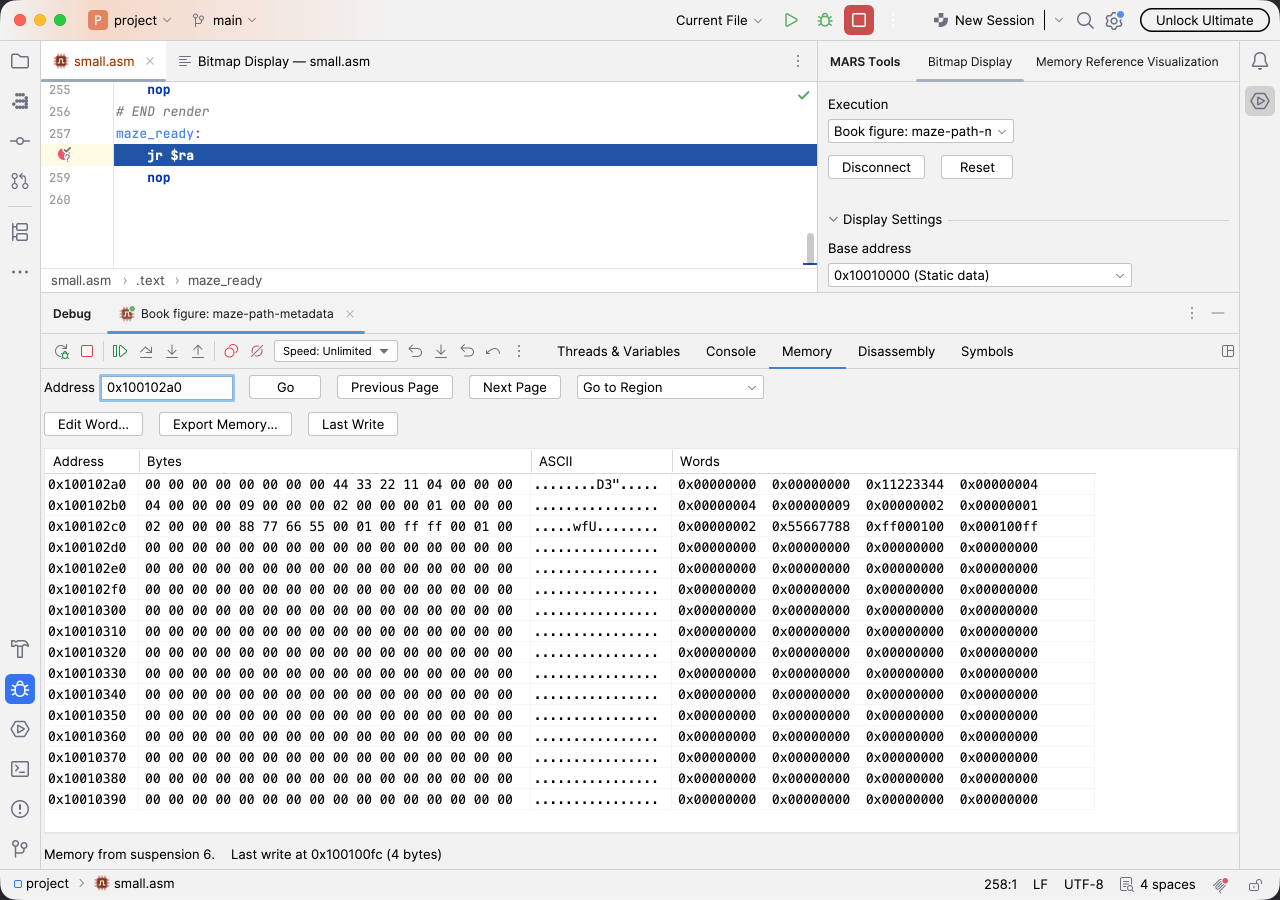
\includegraphics[artifact]{book/captures/010-maze-explorer/f03-path/metadata.png}}
\edef\MARSpathsourceLeft{\the\dimexpr0.036718750\wd0\relax}
\edef\MARSpathsourceBottom{\the\dimexpr0.811111111\ht0\relax}
\edef\MARSpathsourceRight{\the\dimexpr0.611718750\wd0\relax}
\edef\MARSpathsourceTop{\the\dimexpr0.111111111\ht0\relax}
\edef\MARSpathstateLeft{\the\dimexpr0.034375000\wd0\relax}
\edef\MARSpathstateBottom{\the\dimexpr0.422222222\ht0\relax}
\edef\MARSpathstateRight{\the\dimexpr0.584375000\wd0\relax}
\edef\MARSpathstateTop{\the\dimexpr0.497777778\ht0\relax}
\edef\MARSpathlinksLeft{\the\dimexpr0.034375000\wd0\relax}
\edef\MARSpathlinksBottom{\the\dimexpr0.236666667\ht0\relax}
\edef\MARSpathlinksRight{\the\dimexpr0.584375000\wd0\relax}
\edef\MARSpathlinksTop{\the\dimexpr0.616666667\ht0\relax}
\edef\MARSpathplotLeft{\the\dimexpr0.203906250\wd2\relax}
\edef\MARSpathplotBottom{\the\dimexpr0.066666667\ht2\relax}
\edef\MARSpathplotRight{\the\dimexpr0.203906250\wd2\relax}
\edef\MARSpathplotTop{\the\dimexpr0.091111111\ht2\relax}
\edef\MARSpathmemoryLeft{\the\dimexpr0.034375000\wd4\relax}
\edef\MARSpathmemoryBottom{\the\dimexpr0.398888889\ht4\relax}
\edef\MARSpathmemoryRight{\the\dimexpr0.584375000\wd4\relax}
\edef\MARSpathmemoryTop{\the\dimexpr0.497777778\ht4\relax}
\begin{tikzpicture}[alt={Five annotated details at final phase two. All four open cells are processed with state two. Parents connect nine to one to zero and distance nine is two. Route cells are zero, one and nine, colored blue; processed cell eight stays green. Head and tail are four, current nine, result one and route length two.}]
\node[anchor=north west,inner sep=0,font=\small\bfseries] (source-title) at (6mm,0) {Next instruction: return from the renderer};
\node[anchor=north west,inner sep=0] (source) at ([yshift=-1mm]source-title.south west) {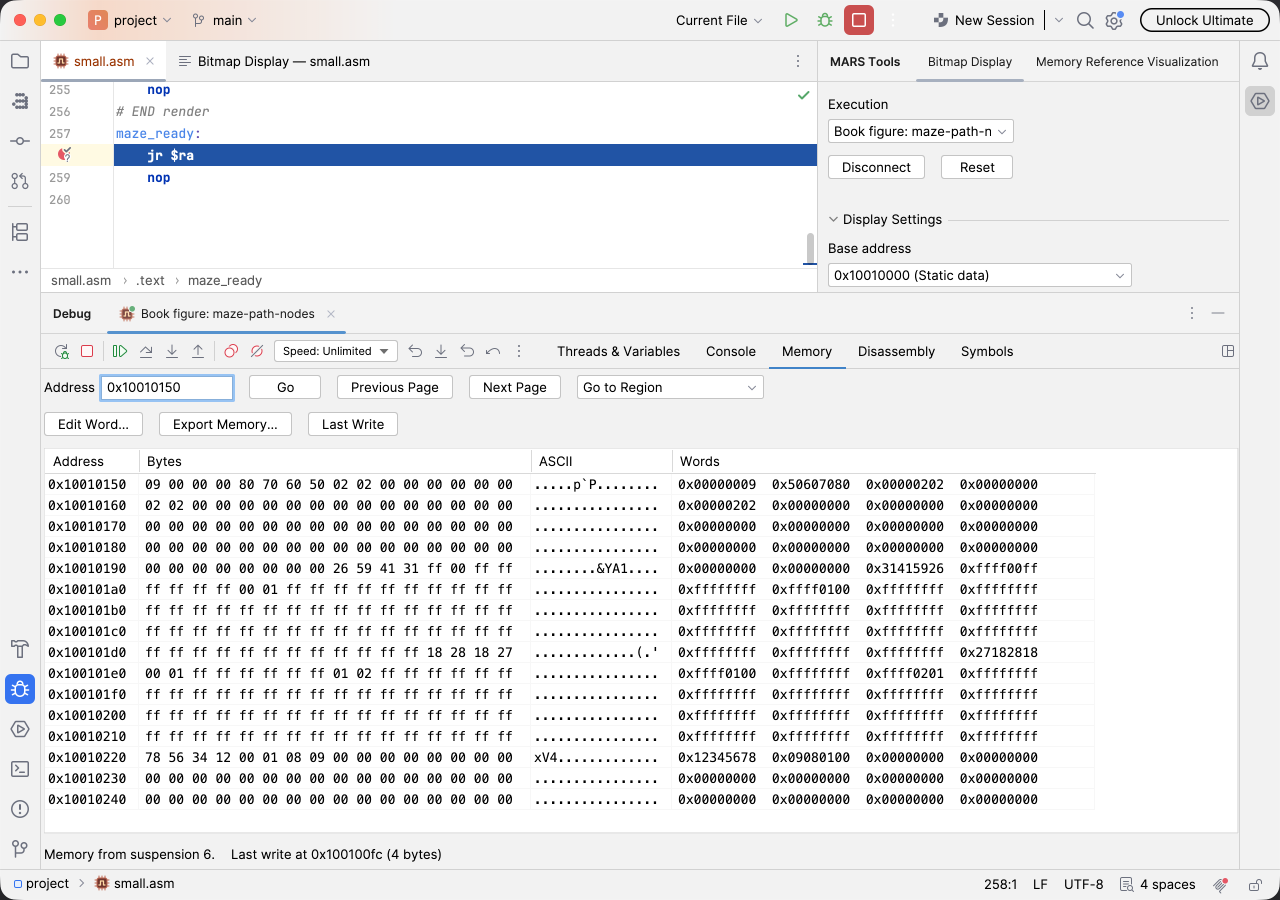
\includegraphics[width=0.7\linewidth,artifact,trim={\MARSpathsourceLeft{} \MARSpathsourceBottom{} \MARSpathsourceRight{} \MARSpathsourceTop{}},clip]{book/captures/010-maze-explorer/f03-path/nodes.png}};
\begin{scope}[shift={(source.south west)},x={($(source.south east)-(source.south west)$)},y={($(source.north west)-(source.south west)$)}]
\draw[black,line width=0.7pt] (0.153333333,0.057142857) rectangle (0.326666667,0.371428571);
\node[draw=black,fill=white,circle,inner sep=1.5pt,font=\footnotesize] at ($(0.153333333,0.371428571)+(-3mm,0)$) {1};
\end{scope}
\node[anchor=north west,inner sep=0,font=\small\bfseries] (state-title) at ([yshift=-1mm]source.south west) {State bytes for the first two rows};
\node[anchor=north west,inner sep=0] (state) at ([yshift=-1mm]state-title.south west) {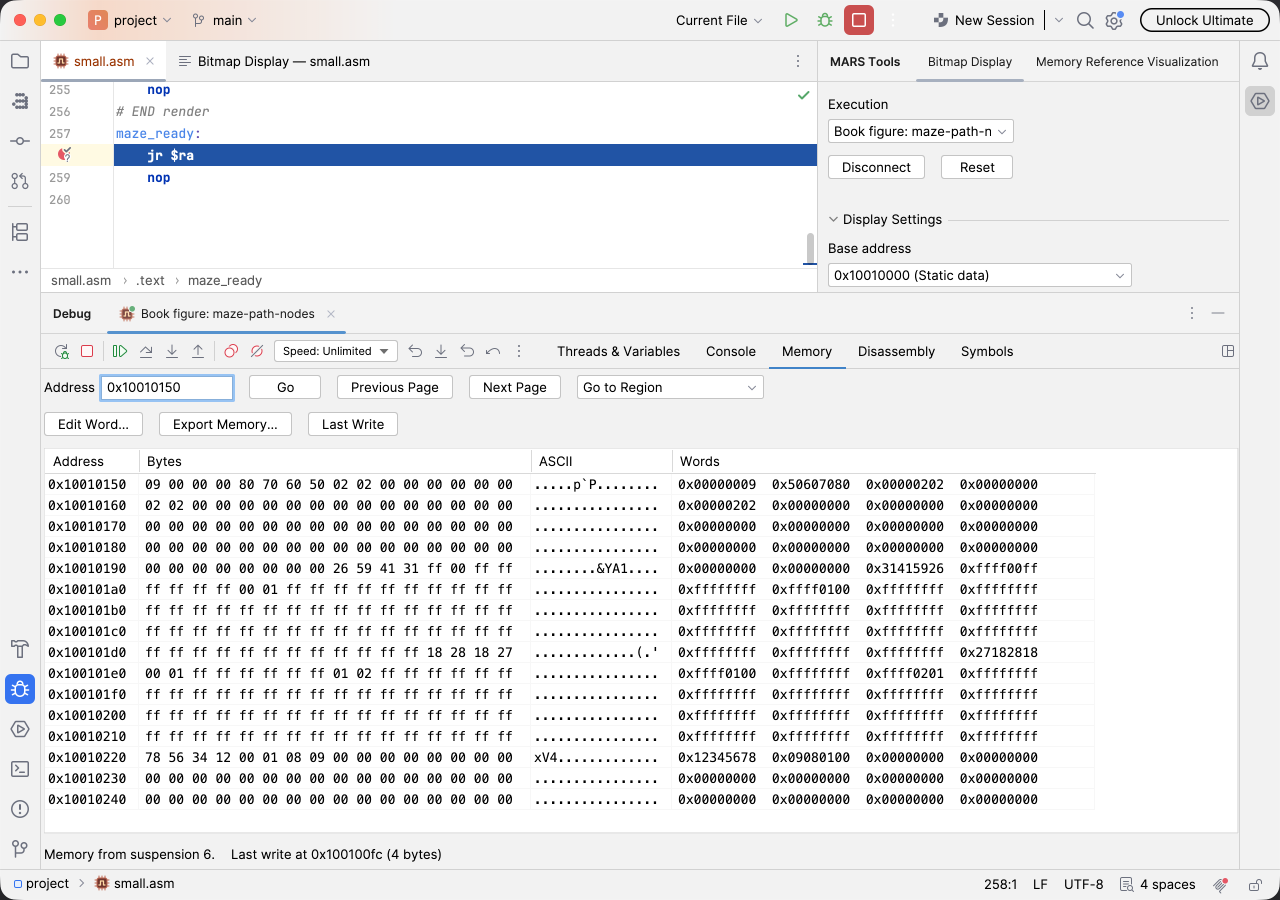
\includegraphics[width=0.78\linewidth,artifact,trim={\MARSpathstateLeft{} \MARSpathstateBottom{} \MARSpathstateRight{} \MARSpathstateTop{}},clip]{book/captures/010-maze-explorer/f03-path/nodes.png}};
\begin{scope}[shift={(state.south west)},x={($(state.south east)-(state.south west)$)},y={($(state.north west)-(state.south west)$)}]
\draw[black,line width=0.7pt] (0.194672131,0.055555556) rectangle (0.997950820,0.638888889);
\node[draw=black,fill=white,circle,inner sep=1.5pt,font=\footnotesize] at ($(0.000000000,0.638888889)+(-3mm,0)$) {2};
\end{scope}
\node[anchor=north west,inner sep=0,font=\small\bfseries] (links-title) at ([yshift=-1mm]state.south west) {Parents and distances};
\node[anchor=north west,inner sep=0] (links) at ([yshift=-1mm]links-title.south west) {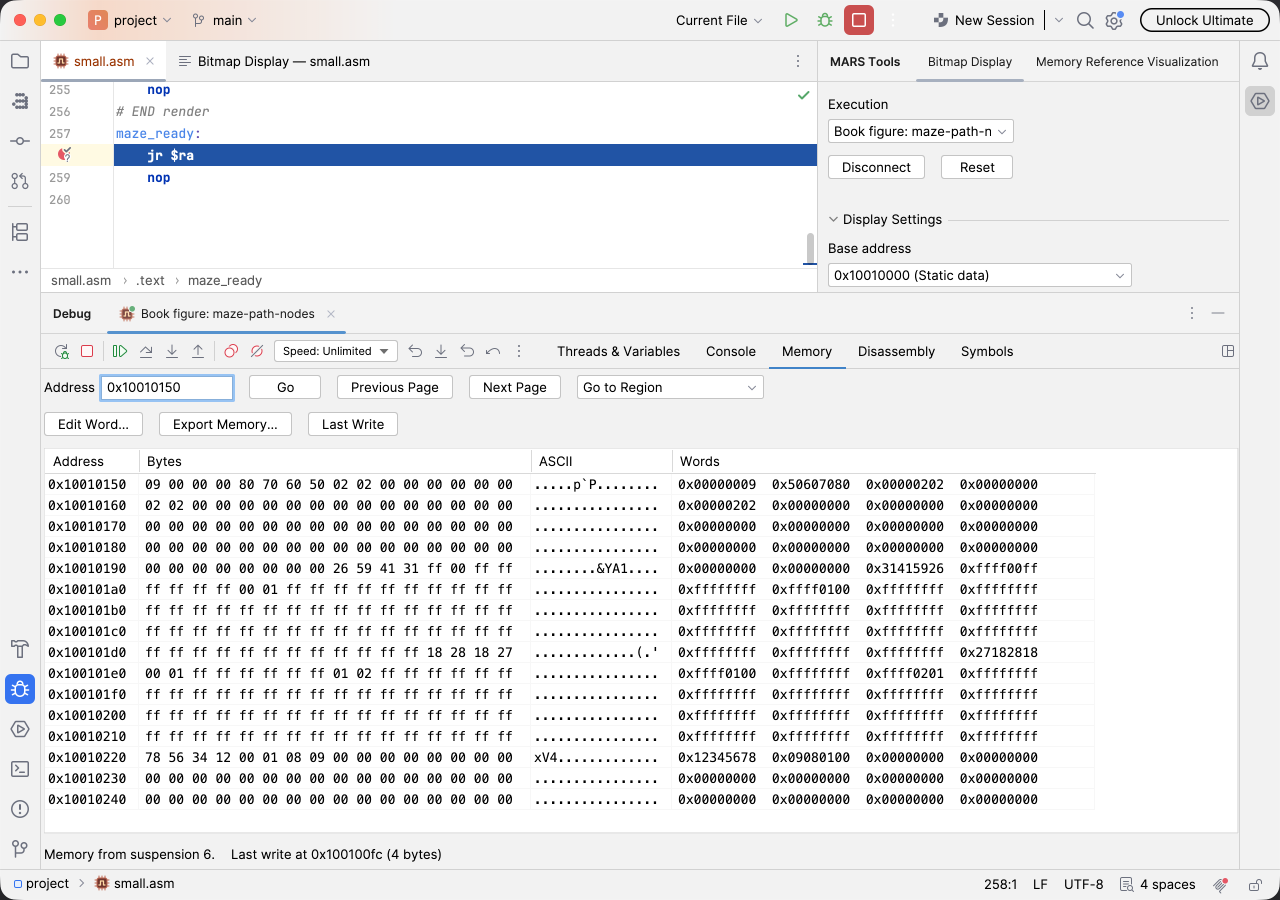
\includegraphics[width=0.6\linewidth,artifact,trim={\MARSpathlinksLeft{} \MARSpathlinksBottom{} \MARSpathlinksRight{} \MARSpathlinksTop{}},clip]{book/captures/010-maze-explorer/f03-path/nodes.png}};
\begin{scope}[shift={(links.south west)},x={($(links.south east)-(links.south west)$)},y={($(links.north west)-(links.south west)$)}]
\draw[black,line width=0.7pt] (0.194672131,0.022727273) rectangle (0.997950820,0.977272727);
\node[draw=black,fill=white,circle,inner sep=1.5pt,font=\footnotesize] at ($(0.000000000,0.977272727)+(-3mm,0)$) {3};
\end{scope}
\node[anchor=north west,inner sep=0,font=\small\bfseries] (plot-title) at ([xshift=0.67\linewidth]links-title.north west) {Published maze cells};
\node[anchor=north west,inner sep=0] (plot) at ([yshift=-1mm]plot-title.south west) {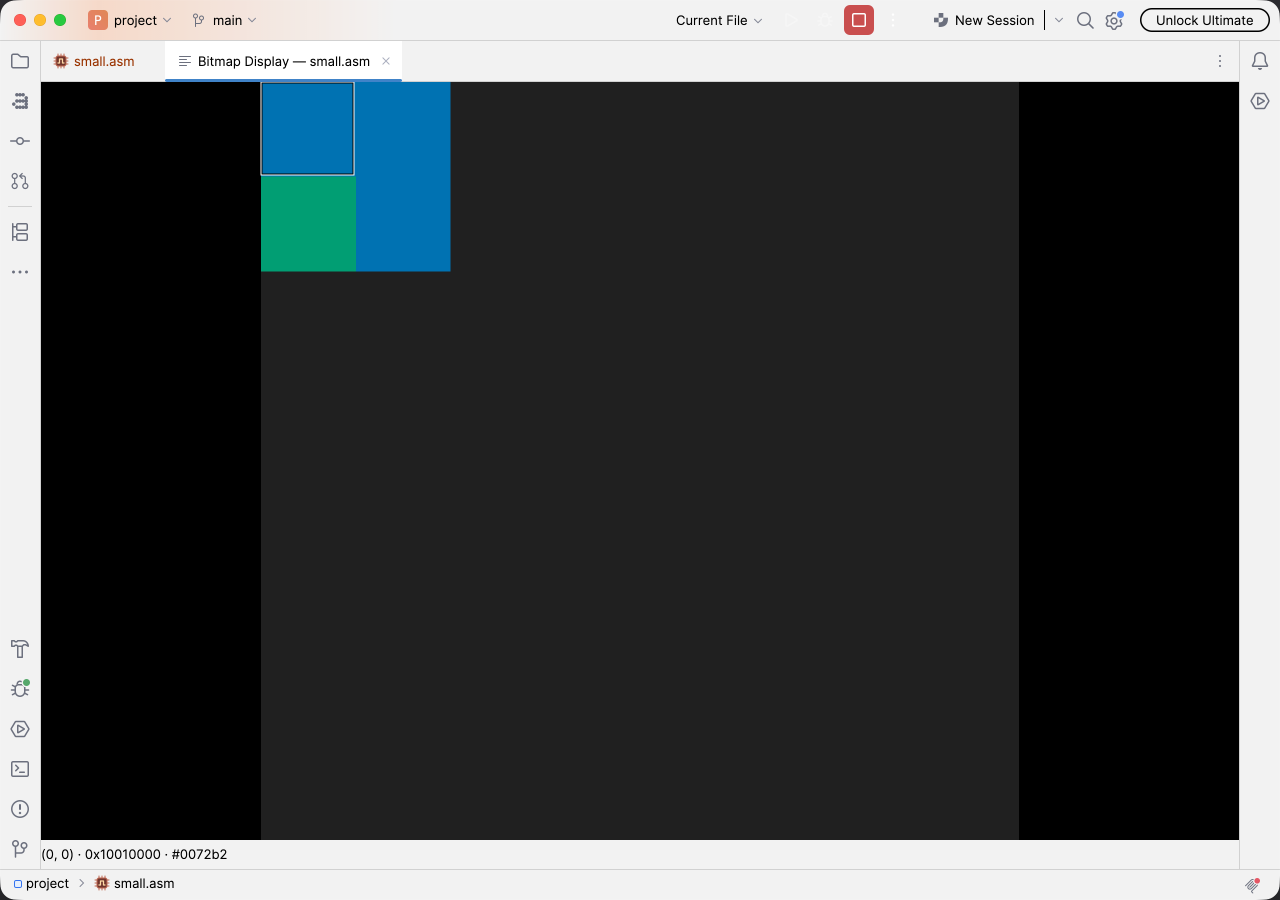
\includegraphics[width=0.27\linewidth,artifact,trim={\MARSpathplotLeft{} \MARSpathplotBottom{} \MARSpathplotRight{} \MARSpathplotTop{}},clip]{book/captures/010-maze-explorer/f03-path/bitmap.png}};
\begin{scope}[shift={(plot.south west)},x={($(plot.south east)-(plot.south west)$)},y={($(plot.north west)-(plot.south west)$)}]
\draw[black,line width=0.7pt] (0.000000000,0.000000000) rectangle (1.000000000,1.000000000);
\node[draw=black,fill=white,circle,inner sep=1.5pt,font=\footnotesize] at ($(0.000000000,1.000000000)+(-3mm,0)$) {4};
\foreach \c in {0,...,7} {\node[anchor=north,font=\scriptsize,inner sep=0] at ({(\c+0.5)/8},-0.035) {\c}; \node[anchor=east,font=\scriptsize,inner sep=0] at (-0.025,{1-(\c+0.5)/8}) {\c};}
\node[anchor=north,font=\scriptsize,inner sep=0] at (0.5,-0.11) {$x$}; \node[anchor=east,font=\scriptsize,inner sep=0] at (-0.10,0.5) {$y$};
\end{scope}
\node[anchor=north west,inner sep=0,font=\small\bfseries] (memory-title) at ([yshift=-9mm]links-title.north west |- plot.south west) {Queue counters and published phase};
\node[anchor=north west,inner sep=0] (memory) at ([yshift=-1mm]memory-title.south west) {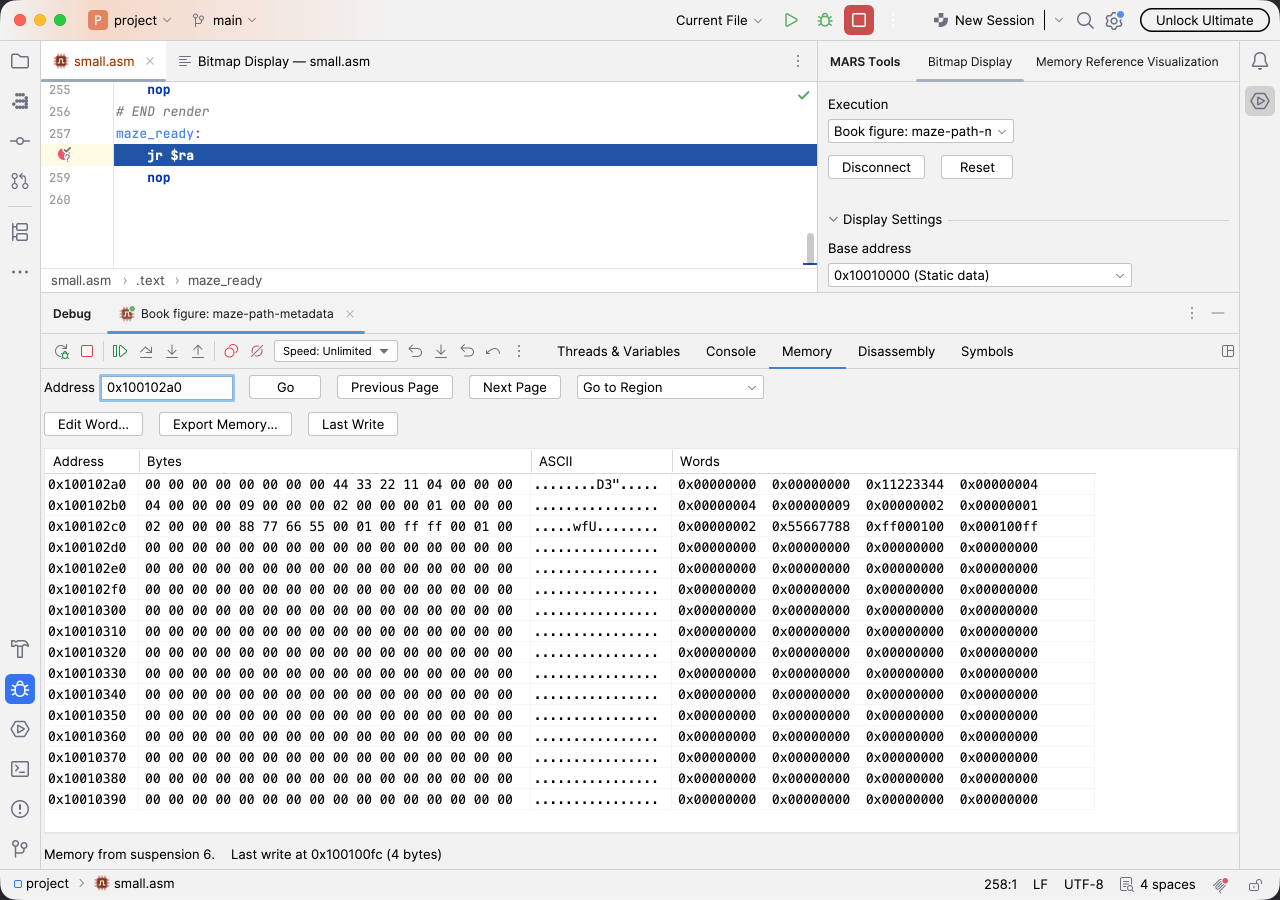
\includegraphics[width=0.78\linewidth,artifact,trim={\MARSpathmemoryLeft{} \MARSpathmemoryBottom{} \MARSpathmemoryRight{} \MARSpathmemoryTop{}},clip]{book/captures/010-maze-explorer/f03-path/metadata.png}};
\begin{scope}[shift={(memory.south west)},x={($(memory.south east)-(memory.south west)$)},y={($(memory.north west)-(memory.south west)$)}]
\draw[black,line width=0.7pt] (0.194672131,0.043010753) rectangle (0.997950820,0.720430108);
\node[draw=black,fill=white,circle,inner sep=1.5pt,font=\footnotesize] at ($(0.000000000,0.720430108)+(-3mm,0)$) {5};
\end{scope}
\end{tikzpicture}
\par\smallskip
\begin{minipage}{\linewidth}
\small
\begin{enumerate}
\item The condition \texttt{word(phase) == 2} selects the final render. The preceding goal-expansion frame had phase 1 and no route overlay, despite having the same head, tail and current values.
\item All four open cells contain state 2. Route membership is a separate \texttt{path} mask; selecting the route does not replace the processed-state bytes.
\item Parent 9 is 1, and parent 1 is 0. Following these bytes backward gives $9\to1\to0$; reversing the chain gives the route $0\to1\to9$. Distance 9 is 2: two edges join three cells.
\item Blue route cells are $(0,0)$, $(1,0)$ and $(1,1)$. Cell $(0,1)$ is processed but outside this route. The equally short route through cell 8 is also valid; this reference\textquotesingle s neighbor order selects cell 1 first.
\item \texttt{head}=\texttt{tail}=4 leaves an empty frontier. \texttt{current}=9, phase 2, result 1 and length 2 publish success. The renderer\textquotesingle s next return leads toward normal exit.
\end{enumerate}
\end{minipage}
\caption{The final small-room publication selects a two-edge shortest route.}
\label{capture:010-maze-explorer-f03-path}
\label{maze-f03-path}
\end{figure}
\par
